\documentclass{ctexart}
\usepackage{geometry}
\usepackage{listings}
\usepackage{textcomp}
\usepackage{graphicx}
\usepackage[hidelinks]{hyperref}
\usepackage{hyperref}
\usepackage{appendix}
\usepackage{multirow}
\usepackage{amsmath,amssymb,amsfonts}
\usepackage[framed,numbered,autolinebreaks,useliterate]{mcode}
%记得用xelatex
% 导入首行缩进用的宏包
\usepackage{indentfirst}
\setlength{\parindent}{2em}
% 每行缩进两个汉字
\usepackage{url}
\setlength{\parindent}{0pt}
\setlength{\parskip}{18pt}
\title{\vspace{+4cm}\textbf{应用数学选讲第一次作业}}
\author{冯健齐 202023092020}
\date{\today}
% //////////////////////////////////////////////////

\begin{document}

\maketitle
%目录
\newpage
\pagenumbering{Roman}
\setcounter{page}{0}
\tableofcontents
\newpage
\setcounter{page}{1}
\pagenumbering{arabic}
%标题

\section{6.1复习题1}
\subsection{等额本息还款计算}
\setlength{\parindent}{2em}用matlb进行计算,代码如下:


\begin{lstlisting}
format long
A=1000000; %贷款总额
n=240; %还款期数
r=5.65*(0.01)/12; %月利率
a=A*r*((1+r)^n/((1+r)^n-1)) %每月还款金额
A1=n*a %还款总额
\end{lstlisting}



\setlength{\parindent}{2em}计算结果为每月还款金额为6963.867690174990元,总还款金额为1671328.245641998元。与网络等额本息计算器进行对比,可知数据正确。

\begin{figure}[h!]
\centering
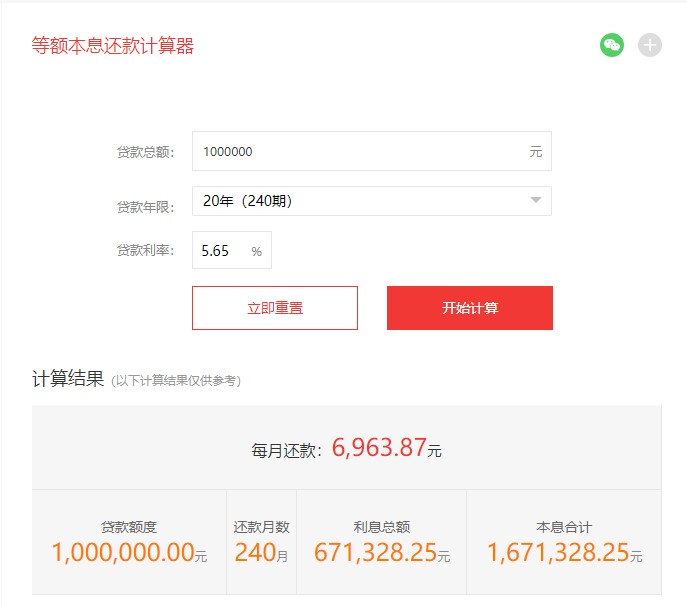
\includegraphics[width=0.68\textwidth]{等额本息.JPG}
\caption{等额本息还款计算器}
\end{figure}



\subsection{等额本金还款计算}
\setlength{\parindent}{2em}用matlb进行计算,代码如下:


\begin{lstlisting}
clc;clear;
format long
A=1000000; %贷款总额
n=240; %还款期数
r=5.65*(0.01)/12; %月利率
x1=A/n+A*r %首月还款金额
xx=A*r/n %每月递减金额
A2=A+A*r*(n+1)/2 %还款总金额
\end{lstlisting}



\setlength{\parindent}{2em}计算结果为第一个月还款8875元,之后每个月还款减少19.618055555555554元,总还款金额为1567354.166666667元。与网络等额本金计算器进行对比,可知数据正确。

\begin{figure}[h!]
\centering
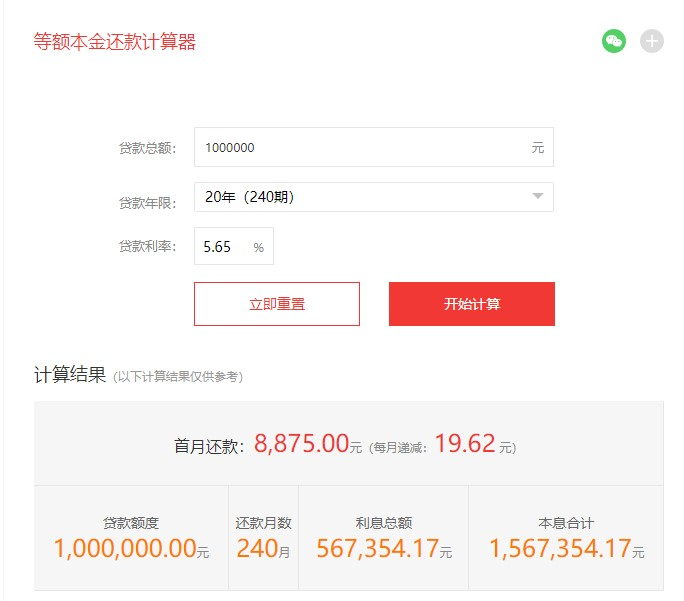
\includegraphics[width=0.68\textwidth]{等额本金.JPG}
\caption{等额本金还款计算器}
\end{figure}


\section{6.1复习题2}

\begin{Large}
\setlength{\parindent}{2em}由公式推导可知,假设借款金额为$x_{0}$,月利率为$r$,贷款期限为$n$,那么有等额本息还款总额$A_{1}$与等额本金还款总额$A_{2}$的公式有



$A_{1}=\frac{x_{0}rn(1+r)^n}{(1+r)^n-1}$ \qquad $A_{2}=x_{0}+\frac{x_{0}r(1+n)}{2}$


即证
$\frac{x_{0}rn(1+r)^n}{(1+r)^n-1}>x_{0}+\frac{x_{0}r(1+n)}{2}$

$\Leftrightarrow 2rn(1+r)^n>2(1+r)^n-2+r(1+n)(1+r)^n-r(1+n)$

$\Leftrightarrow (rn-2-r)(1+r)^n>-r-rn-2$

设函数$f(r,n)=(rn-2-r)(1+r)^n+rn+r+2$,即证对$r\isin(0,1),n\isin(1,+\infty)$成立。


对函数求导得


$f_{r}^{\prime}(r,n)=(n-1)(1+r)^n+n(rn-r-2)(1+r)^{n-1}+n+1$

$=(1+r)^{n-1}[(1+r)(n-1)+nr(n-1)-2n]+n+1$

$=(1+r)^{n-1}(-n-1-r+nr^2)+n+1$

$=(1+r)^{n-1}[-(n+1)-r(1+n)(1-n)]+n+1$

$=(n+1)[(1+r)^{n-1}(rn-r-1)+1]$

记其中$h(r,n)=(1+r)^{n-1}(rn-r-1)+1$

对其求导,有

$h_{r}^{\prime}(r,n)=(n-1)(1+r)^{n-2}(rn-r-1)+(1+r)^{n-1}(n-1)$

$=rn(n-1)(1+r)^{n-1}>0$恒成立

故$h(r,n)>h(0,n)=0$,即$f_{r}^{\prime}(r,n)>0$恒成立,即$f(r,n)$在$r\isin(0,1)$上单调递增,$f(r,n)>f(0,n)=0$故$f(r,n)>0$对$r\isin(0,1),n\isin(1,+\infty)$恒成立,即$A_{1}>A_{2}$恒成立。
\end{Large}

\section{6.3代码实现}
\subsection{市场经济中物价波动模型}
由课本P199中(4)式与(1)式可得下面模型并进行计算与绘图。

\begin{lstlisting}
clc;clear;
%6.3市场经济中的物价波动
%x差分方程为
a = 0.1; %设置初始状态
b = 5; %设置初始状态
k = 10; %设置初始次数
x_0 = 100; %设置初始状态
x_1 = 110; %设置初始状态
y_0 = 10; %设置初始状态
x = x_1 * ones(1,k);
y = ones(1,k);
for i = 2:k
    x(i) = (- a * b ) ^ ( i - 1 ) * ( x_1 - x_0 ) + x_0;
end
for j = 1:k
    y(j) = - a * ( x(j) - x_0 ) + y_0 ;
end
%绘制x
plot( 1:k , x );
grid on;
title(['a=', num2str(a) , ',' , 'b=', num2str(b) , '时差分方程图像']);
xlabel('k');
ylabel('x(k)');
%绘制y
plot( 1:k , y );
title(['a=', num2str(a) , ',' , 'b=', num2str(b) , '时差分方程图像']);
xlabel('k');
ylabel('y(k)');
grid on;
\end{lstlisting}

\begin{figure}[htbp]
\centering
\begin{minipage}[t]{0.48\textwidth}
\centering
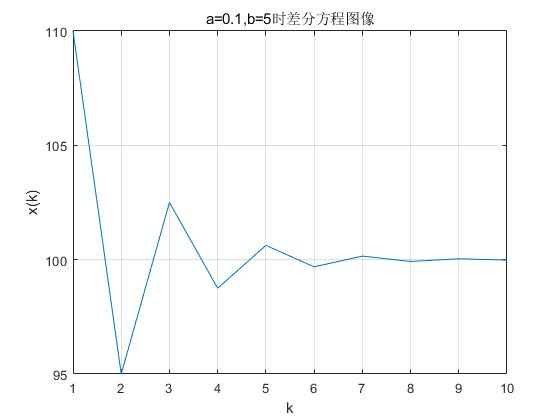
\includegraphics[width=8cm]{x1.jpg}
\end{minipage}
\begin{minipage}[t]{0.48\textwidth}
\centering
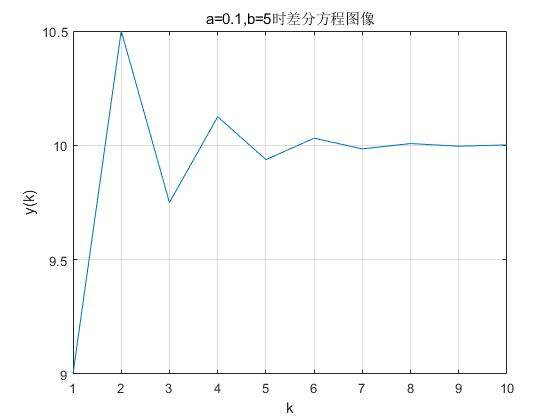
\includegraphics[width=8cm]{y1.jpg}
\end{minipage}
\end{figure}

\begin{lstlisting}
%改变参数再次绘制
a = 0.24; %设置初始状态
b = 5; %设置初始状态
k = 10; %设置初始次数
x_0 = 100; %设置初始状态
x_1 = 110; %设置初始状态
y_0 = 10; %设置初始状态
x = x_1 * ones(1,k);
y = ones(1,k);
for i = 2:k
    x(i) = (- a * b ) ^ ( i - 1 ) * ( x_1 - x_0 ) + x_0;
end
for j = 1:k
    y(j) = - a * ( x(j) - x_0 ) + y_0 ;
end
%绘制x
plot( 1:k , x );
grid on;
title(['a=', num2str(a) , ',' , 'b=', num2str(b) , '时差分方程图像']);
xlabel('k');
ylabel('x(k)');
%绘制y
plot( 1:k , y );
title(['a=', num2str(a) , ',' , 'b=', num2str(b) , '时差分方程图像']);
xlabel('k');
ylabel('y(k)');
grid on;
\end{lstlisting}

\begin{figure}[htbp]
\centering
\begin{minipage}[t]{0.48\textwidth}
\centering
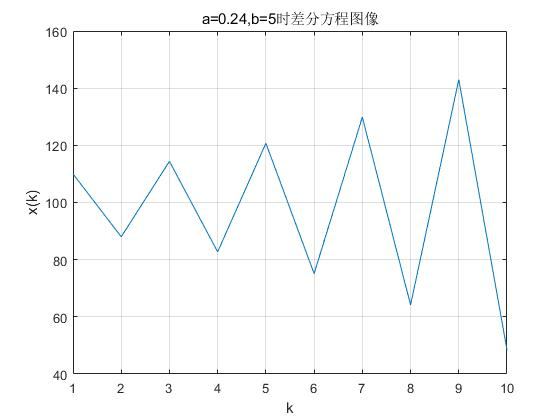
\includegraphics[width=8cm]{6.1x.jpg}
\end{minipage}
\begin{minipage}[t]{0.48\textwidth}
\centering
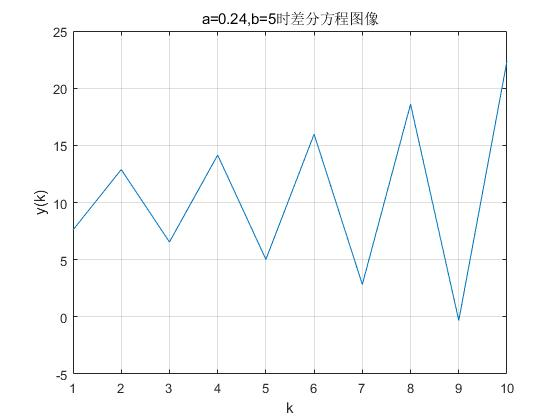
\includegraphics[width=8cm]{6.1y.jpg}
\end{minipage}
\end{figure}

\subsection{物价波动模型的推广}
由课本P202中(7)式与之前式子可得下面模型并进行计算与绘图。
\begin{lstlisting}
clc;clear;
%6.3推广
a = 0.24; %设置初始状态
b = 5; %设置初始状态
k = 16; %设置初始次数
x_0 = 100; %设置初始状态
x_1 = 110; %设置初始状态
x_2 = 88; %设置初始状态
y_0 = 10; %设置初始状态
x = ones(1,k);
x(1) = x_1;
x(2) = x_2;
y = ones(1,k);
for i = 3:k
    x(i) = (- a * b ) * ( (x( i - 1 ) + x(i - 2))/2 - x_0 ) + x_0;
end
for j = 1:k
    y(j) = - a * ( x(j) - x_0 ) + y_0 ;
end
%绘制x
plot( 1:k , x );
grid on;
title(['a=', num2str(a) , ',' , 'b=', num2str(b) , '时推广差分方程图像']);
xlabel('k');
ylabel('x(k)');
%绘制y
plot( 1:k , y );
title(['a=', num2str(a) , ',' , 'b=', num2str(b) , '时推广差分方程图像']);
xlabel('k');
ylabel('y(k)');
grid on;
\end{lstlisting}

\begin{figure}[htbp]
\centering
\begin{minipage}[t]{0.48\textwidth}
\centering
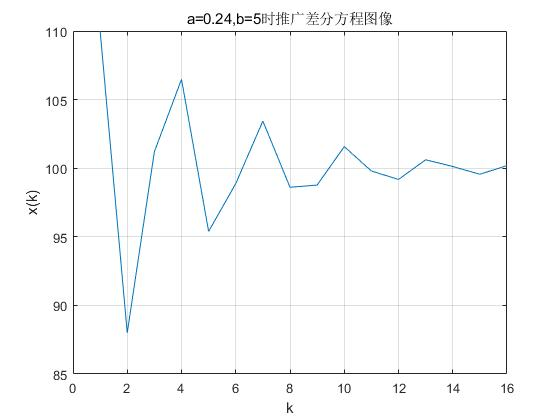
\includegraphics[width=8cm]{x2.jpg}
\end{minipage}
\begin{minipage}[t]{0.48\textwidth}
\centering
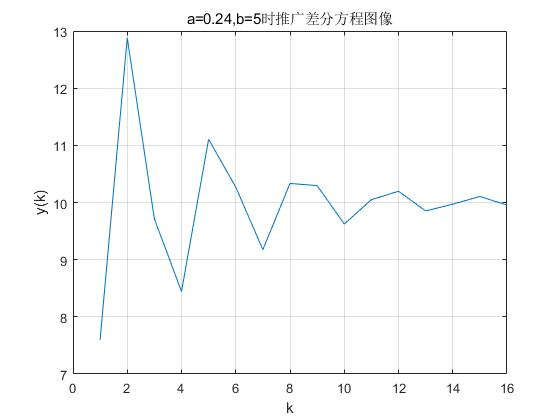
\includegraphics[width=8cm]{y2.jpg}
\end{minipage}
\end{figure}


\section{6.4代码实现}
由课本P204中(4)式与(5)式可得下面模型并进行计算与绘图。
\begin{lstlisting}
clc;clear;
%6.4动物的繁殖与收获
k = 30;
s = [ 0.5 0.8 0.8 0.1 ];
b = [ 0 0.2 1.8 0.8 0.2 ];
L = [ b ; [ diag(s) , zeros(length(s),1) ] ];
x = 100 * ones( 5 , k + 1 );
y = x;
%draw x
for i = 2 : k + 1
    x(:,i) = L * x(:,i-1);
end
plot( [ 0 , 1:k ] , x );
grid on;
title('x(k)的图像( 从下往上为x1(k)-x5(k) )');
xlabel('k');
ylabel('各个x(k)');
%draw x*
for i = 1 : k + 1
    y(:,i) = x(:,i) / sum(x(:,i));
end
plot( [ 0 , 1:k ] , y );
grid on;
title('x*(k)的图像( 从下往上为x*1(k)-x*5(k) )');
xlabel('k');
ylabel('各个x*(k)');
\end{lstlisting}
\begin{figure}[htbp]
\centering
\begin{minipage}[t]{0.48\textwidth}
\centering
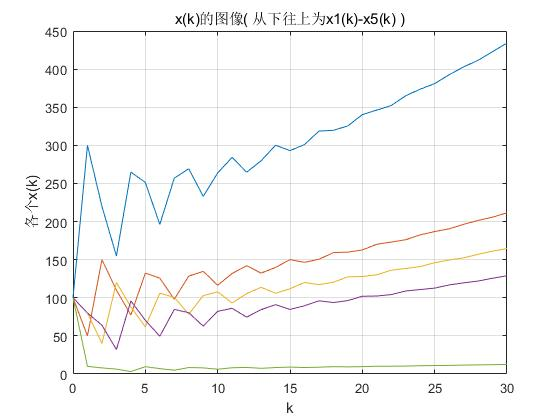
\includegraphics[width=6cm]{xk.jpg}
\end{minipage}
\begin{minipage}[t]{0.48\textwidth}
\centering
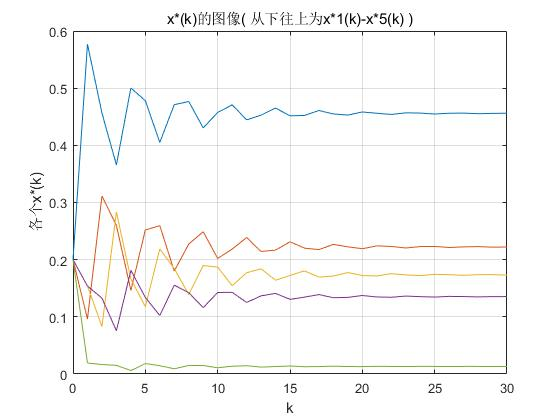
\includegraphics[width=6cm]{xkk.jpg}
\end{minipage}
\end{figure}

\end{document}



